%こねこ。のテンプレート(ver 2.3)
%Copyright © 2021-2022 こねこ。 All Rights Reserved.

\documentclass[a4paper, 9pt]{jsarticle}
\usepackage[top=20truemm, bottom=20truemm, left=20truemm, right=20truemm]{geometry}

\usepackage{preamble}
%日本語を使うときは必須
\usepackage{jpreamble}
%化学用追加パッケージ
\usepackage{prechemistry}
%情報用追加パッケージ
\usepackage{preprog}
%フォント操作用追加パッケージ
\usepackage{prefonts}

\title{\sf{こねこ。のテンプレートver2.3使用方法}}
\author{\sf{こねこ。}}
\date{\sf{\today}}
\begin{document}
\maketitle
こねこ。のテンプレートの使い方のうちよく使うものを,実際にこのtexファイルで使うことにより紹介しています.texファイルをいじったときにPDFが改変されて説明が読めなくなってしまう事故を防ぐために,PDFに関してはバックアップをとってあります.\par 
\section{準備}
\tt{preamble.sty},\tt{preamblej.sty},\tt{prechemistry.sty},\tt{preprog.sty},\tt{prefonts.sty},を以下の場所にコピーしたのち,その場所に移動してから\tt{mktexlsr}コマンドを実行してください.\footnote{Linux用はないのか,などと言う人が必ずいますが,Linuxなんて物好きなものを使ってる人ならこの程度の処理は自分でコマンドで済ませたいと思いますのでつくりませんでした.みんな,Ubuntu使おうぜ.}
\arki{
	\item Windowsの場合:\tt{C:/texlive/texmf-local/tex/platex/}
 \item Macの場合:\tt{/Users/ユーザー名/Library/texmf/tex/platex/}
}
また,Windowsの場合は同封の\tt{win\_install.bat}を実行する(ダブルクリック)ことにより上記の処理を行うことができます.また,Macの場合,同封の\tt{mac\_install}を実行する(ターミナルを開き,\tt{cd}を用いて\tt{mac\_install}がある場所へ移動したのち\tt{./mac\_install}と打つ)ことにより上記の処理を行うことができます.中は以下のようになっています.
\lstinputlisting{../../win_install.bat}
\lstinputlisting{../../mac_install}

\section{preamble.sty}
ドキュメントを読み出すときに必ず使用するstyファイルです.
\subsection{General}
よく使うパッケージを\tt{usepackage}してあります.数式を扱うためのパッケージはもちろんのこと,例えば\url{google.co.jp}のようにURLを貼り付ける\tt{url}パッケージや,\uwave{波線}などを使う\tt{ulem}パッケージなどが使えます.本来URLは\tt{google.co.jp}のようなフォントで表されますが,見栄えが悪いのでromanフォントになるように\tt{renewcommand}してあります.
\subsection{ドキュメントのレイアウト}
コメントオフにしてありますが,それぞれの値を適切にいじることによりテキストのマージンなどを操作することができます.
\subsection{雑部}
番号や色についての設定です.例えば\shikaku{1}や\ctext{1}のように使います.色を変えるときは\red{このようにすれば赤になります}.\blue{青や}\green{緑},\yellow{黄色も}使用できます.見辛いですけどね.
\subsection{画像・グラフ}
\fig{重力加速度の実験図}{pic1}{0.3}{kigu.eps}
とすると,画像を読み出すことができます.\tt{0.3}の部分は倍率を表しているので,大きくしたいときにはもっと大きくしてみましょう.\tt{preambles.sty}にある\tt{\graphicspath}を適切に変更することで,画像のフォルダを参照できます.表は,例えば次のように書きます.
\tab{実験データ}{tab1}{ccc}{
	小球の直径  & 小球の半径 &KEからスケールまでの距離\\
$D/\rm{mm}$ & $r/\rm{mm}$ & $L/\rm{mm}$ \\
 \hline
25.4$\pm$0.05&12.7$\pm$0.03&881.9\\
25.4$\pm$0.05&12.7$\pm$0.03&881.7\\
25.4$\pm$0.05&12.7$\pm$0.03&881.6\\
 \hline
}
\subsection{数式}
\eq{ma=F}{eq1}
とすると,数式が書けます.また,
\alg{
    \int_0^{2\pi}\sin{2x}\cos{nx}dx\nonumber\\
    =& \int_0^{2\pi}\frac{1}{2}\left\{\sin(2x+nx)+\sin{(2x-nx)}\right\}dx\nonumber\\
    =& \frac{1}{2}\left[-\frac{1}{2+n}\cos{(2x+nx)}-\frac{1}{2-n}\cos{(2x-nx)}\right]_0^{2\pi} = 0
}{eq2}
とすると,複数行の式が書けます.通し番号をなくしたい場合は,
\algg{
	\int_0^{2\pi}\sin{2x}\cos{nx}dx\nonumber\\
    =& \int_0^{2\pi}\frac{1}{2}\left\{\sin(2x+nx)+\sin{(2x-nx)}\right\}dx\nonumber\\
    =& \frac{1}{2}\left[-\frac{1}{2+n}\cos{(2x+nx)}-\frac{1}{2-n}\cos{(2x-nx)}\right]_0^{2\pi} = 0
}
が便利です.\tt{alg}では必ずラベルを貼ることになります.\par 
例えば,
\eq{\lim_{x\rightarrow a}b \defarrow \forall\epsilon>0, \exists\delta>0;\forall x\in\bb{R}[|x-a|<\delta \Rightarrow |f(x)-b| <\epsilon] }{eq3}
は,
\eq{\lim_{x\rightarrow a}b \defeq \forall\epsilon>0, \exists\delta>0;\forall x\in\bb{R}[|x-a|<\delta \Rightarrow |f(x)-b| <\epsilon] }{eq4}
とも
\eq{\lim_{x\rightarrow a}b \defeqq\forall\epsilon>0, \exists\delta>0;\forall x\in\bb{R}[|x-a|<\delta \Rightarrow |f(x)-b| <\epsilon] }{eq5}
とも書きます.大学によっては$\asin{x}\defeq\arcsin{x}$というところもありますよね.\par 
\eq{\det\pmt{a&b\\c&d} = \det\bmt{a&b\\c&d} = \vmt{a&b\\c&d}=ac-bd}{eq6}
は覚えているでしょうか.また,
\eq{\bmt{\general{b}{i}{j}{m}{n}}}{eq7}
とすると,一般の行列を簡単に書くことができます.ブロック行列はあまり使わないのでとりあえず置いておきましょう.\par 
例えば,
\eq{f(x) = \left\{\ar{1/x\\2}\right.}{eq8}
と書くこともありますが,空白を大きくしたいときもあります.このときは,
\eq{f(x) = \left\{\Ar{2.0}{1/x\\2}\right.}{eq9}
とすると間の空白が大きくなりました.さらに,
\eq{f(x) = \left\{\arr{ll}{1/x&(x<0)\\2&(x\geq 0)}\right.}{eq10}
\eq{f(x) = \left\{\Arr{ll}{2.0}{1/x&(x<0)\\2&(x\geq 0)}\right.}{eq11}
とすれば,場合分けもわかりやすく表示できます.\par 
微分記号はいちいち書くのめんどくさかったりしますよね.dがRomanなので.
\algg{
	\rmd{y}{x} &= x\\
	\d y &= x\d x\\
	y &= \frac{1}{2}x^2 + Const.
}
のように書きます.もちろん偏微分もあります.普通の微分・偏微分ともに1階,2階の微分まで用意してあります.
\eq{\ptdd{f}{t} = v^2\ptdd{f}{x}}{eq12}

\subsection{自然科学}
単位は$12\ut{V}$のように書くと,間に適度なスペースが保たれます.いまは数式で囲みましたが,そのままでも書けます(12\ut{V}).セルシウス度は35\ut{\C}のように書きましょう.また,有効数字のあるものは$\signi{1}{2}$のように書きます.文中で書くことが多いものでもあるので,\signi{1}{2}\ut{\C}のように数式中でなくても書けるようにしてあります.

\subsection{tikz}

\tt{circuitikz}を使うと,このように回路図が書けます.
\begin{figure}[H]
  \begin{center}
    \begin{circuitikz}[american currents]
    \ctikzset{bipoles/oscope/waveform=sin}
 \draw (0,0)
 to[short](0,3)
    to[european resistor=$R$] (3,3)
to[L=$L$] (5,3)
to[C=$C$] (7,3)
to[short](7,0)
to[short](6,0)
 to[battery1](4,0)
 to[short] (0,0);
    \end{circuitikz}
    \label{kairo}
    \caption{RLC直列回路}
  \end{center}
\end{figure}

\tt{pgfplots}を使うと,このようにグラフが書けます.いい感じになるように軸などを設定しておきましたが,その設定に関する説明は特にしません.自分で調べてみてください.
\begin{figure}[H]
	\centering
	\begin{tikzpicture}
	\begin{axis}[
	compat = newest,
	xmin = 0, xmax =265, 
	ymin = -3, ymax =0, 
	%xtick distanceを変えることにより,主目盛の大きさを変えることができます
	xtick distance = 50, 
	minor x tick num = 4, 
	%ytick distanceを変えることにより,主目盛の大きさを変えることができます
	ytick distance = 0.5, 
	minor y tick num = 4, 
	xlabel = {時刻$t/\mu s$}, ylabel = {対数値$\ln{(V/V_0)}$},
	enlarge x limits = false]
	\addplot[black!55!black, mark = *, only marks]table{
	0.0 0.0
	48.0 -0.455062049
	97.0 -0.921681581
	146.0 -1.354545663
	195.0 -1.824549292
	241.0 -2.2300144
	};
	\addplot[samples = 200, domain = -1:266]{-0.009309872155860146* x};
	\end{axis}
	\end{tikzpicture}
	\caption{実験1における時刻$t/\mu s$と対数値$\ln{(V/V_0)}$の関係}
	\label{graph1}
\end{figure}
わかる人にはわかりますが,\tt{addplot}の中の数値を\tt{csv}読み出しなどでプログラムすると,わざわざ打ち込まなくてもグラフを書くことが可能です.\par 
tikzに関するテンプレートはこのtexファイルの下にまとめてあるので適宜使ってください.
\subsection{簡単なフォント操作}
$\rm{latex}$,\bf{latex},\sf{latex},\tt{latex},$\bb{LATEX}$など.
\subsection{セクション記号}
括弧付きで式番号を呼び出すときは,\ref{eq1}のようにします.また,\refeq{eq1},\reffig{graph1},\reftbl{tab1}のように使えるので,使ってみてください.単に\tt{ref}だけよりも使いやすいと思います.\par 
また,定理や定義の表示を直してあります(もともとは英語).
\begin{theorem}
	これが定理です.
\end{theorem}
と書くと,定理や定義に通し番号を勝手に通してくれます.また,
\thm{これが定理です.}
\defi{あ}
\que{い}
\ex{う}
\prc{え}
とも書けます.\par 
四角で囲みたい場合は,このようにします.
\Thm{
これが囲った定理です.
}
証明は末尾に四角がつきます.
\prf{私はこの問いに対する驚くべき証明を思いついたが,余白が狭すぎて書くことができない.}
\Prf{私はこの問いに対する驚くべき証明を思いついたが,余白が狭すぎて書くことができない.}
解答も同様に,次のように書きます.
\ans{これが解答です.}
\Ans{これが解答です.}
まだまだ他にも「系」「補題」などを追加しようと思っています.
\subsection{箇条書き}
renewcommandで「labelenumi」を使う場合「\tt{arki}\{箇条書きの中身\}」,renewcommandで「labelenumii」を使う場合「\tt{arkii}\{箇条書きの中身\}」のように使います.
\arki{
	\item a
 \item \apkii{
	 \item a
  \item \rmkiii{
		\item a
  \item \alphiv{
		\item a
	}
	}
 }
}
\romani{
	\item a
}
また,新しい箇条書きをつくりたいときはこのようにします.
\eni{\gt{問題}\arabic{enumi}}{
	\item a
}
\section{jpreamble.sty}
\tt{textgt}のみ別にしてあります.これは\tt{jarticle}ではなく\tt{article}を使うことになっても\tt{preamble.sty}を使用できるようにしたためです.使い方は\gt{こんな感じ}です.

\section{prechemistry.sty}
ベンゼン環が書けます.また,\tt{mhchem}はめちゃくちゃ使いやすいです.\par 
\eq{\ce{2\phenyl{CH3} + H2 -> \benzene{} + CH4}}{eq13}

\section{prefonts.sty}
オリジナルのフォントを使いたいときに使うシートです.ファイルによってフォントを変えたい場合は,このtexファイルと同じ場所に\tt{prefonts.sty}を置いた方がいろいろやりやすいかも知れません.\par 
全角文字をカウンターにしたいことがあるかも知れないので,いろは,カナ,かな,全角数字,全角アルファベット大文字,全角アルファベット小文字についてカウンターを載せてあります.\par 
フォントを変更する際は,\tt{texmf/fonts}にあるディレクトリのうちそのフォントに適切なディレクトリを選び,その中にフォントファイルを入れることで読み出しが出来るようになります.あらかじめ\LaTeX の中で読み出し可能なフォントに関しては\tt{pxchfon}の前の[]の中にフォント名を入れることで読み出すことができます.そうでないフォントに関しては,\tt{setminchofont}や\tt{setgothicfont}の中にフォントファイルを入れることで読み出すことができます.\tt{setminchofont}や\tt{setgothicfont}に関しては\LaTeX の中で読み出し可能なフォントにも使えるので,明朝体やゴシック体をそれぞれ個別に変更したいときに使えます.

\section{preprog.sty}
プログラムを貼り付けたい場合,あとからそのプログラムを修正してもわざわざコピペし直さなくてよいように,プログラムそのものを読み出して貼り付けてくれます.読み出したいプログラムは\tt{files}というディレクトリを作ってそこに置いてください.相対参照が使えます.
\lstinputlisting{test.c}
\end{document}

%%%%%%%%%%%%%%%%%%%%%%%%%%%%%%%%%%%%%%%%%%%%%%%%%%%%%%%%%%%%%%%%%%%
%%%%%%%%%%%%%%%%%%%%%%%%%%%%%%%%%%%%%%%%%%%%%%%%%%%%%%%%%%%%%%%%%%%%%%%%%%%%%%%%%%%%%%%%%%%%%%%%%%%%%%%%%%%%%%%%%%%%%%%%%%%%%%%%%%%%%%%%%%%%%%%%%%%%%%%%%%%%%%%%%%%%%%%%%%%%%%%%%%%%%%%%%%%%%%%%%%%%%%%%%%%%%%%%%%%%%%%%%%%%%%%%%%%%%%%%%%%%%%%%%%%%%%%%%%%%%%%%%%%%%%%%%%%%%%%%%%%%%%%%%%%%%%%%%%%%%%%%%%%%%%%%%%%%%%%%%%%%%%%%%%%%%%%%%%%%%%%%%%%%%%%%%%%%%%%%%%%%%%%%%%%%%%%%%%%%%%%%%%%%%%%%%%%%%%%%%%%%%%%%%%

簡単なTikZテンプレート
参考:https://math-note.xyz/latex/tikz/tikz-line/

\begin{tikzpicture}
 \draw[->,>=stealth,semithick] (-2,0)--(2,0)node[above]{$x$}; %x軸
 \draw[->,>=stealth,semithick] (0,-1)--(0,3)node[right]{$y$}; %y軸
 \draw (0,0)node[below right]{O}; %原点
 \draw (-1,0)node[below]{$-1$}; %点(-1,0)
 \draw (0,1)node[right]{$1$}; %点(0,1)
 \draw[samples=1000, very thick,domain=#1] plot(#2, {#3})node[right]{$y=#4$};
\end{tikzpicture}

%媒介変数
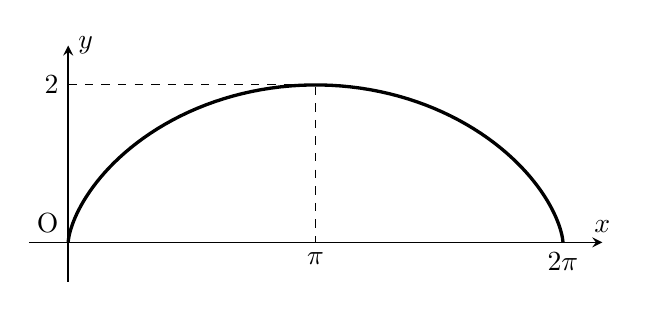
\begin{tikzpicture}
 \draw[->,>=stealth,semithick] (-0.5,0)--(2*pi+0.5,0)node[above]{$x$}; %x軸
 \draw[->,>=stealth,semithick] (0,-0.5)--(0,2.5)node[right]{$y$}; %y軸
 \draw (0,0)node[above left]{O}; %原点
\draw[very thick,samples=100,domain=0:2*pi,variable=\t] plot({\t-sin(\t r)},{1-cos(\t r)}); %サイクロイド%サイクロイド
 \draw (2*pi,0)node[below]{$2\pi$}; %点(2\pi,0)
 \draw[dashed] (0,2)node[left]{2}--(pi,2)--(pi,0)node[below]{$\pi$}; %点(\pi,2)
\end{tikzpicture}

%極座標
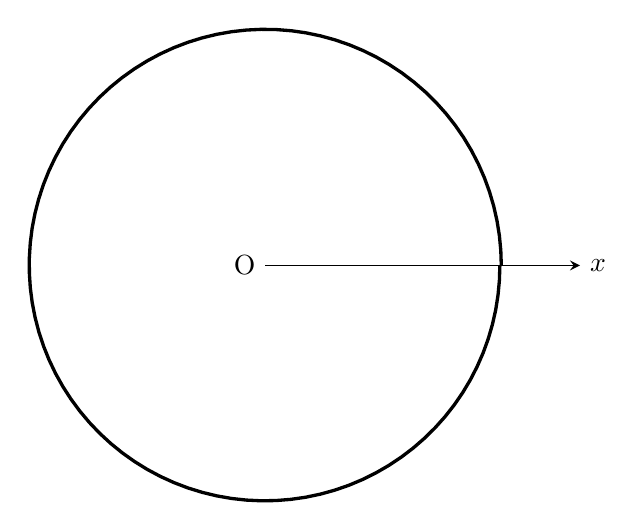
\begin{tikzpicture}
 \draw[->,>=stealth,semithick] (0,0)--(4,0)node[right]{$x$}; %始線
 \draw (0,0)node[left]{O}; %極
 \draw[very thick,samples=100,domain=0:2*pi,variable=\theta] plot(\theta r:{2*1.5*cos(\theta)}); %点(1.5,0)を中心とする半径1.5の円
\end{tikzpicture}

%円弧
\begin{tikzpicture}
 \draw[->,>=stealth,semithick] (-1.5,0)--(2.5,0)node[above]{$x$}; %x軸
 \draw[->,>=stealth,semithick] (0,-0.5)--(0,1)node[right]{$y$}; %y軸
 \draw (0,0)node[above left]{O}; %原点
 \draw (2,1)node[right]{A}; %点A(2,1)
 \draw[very thick] (2,1) arc (60:110:3); %点Aが偏角60度の点であるような半径3の円の,偏角60度から110度の部分の円弧
 \draw (2,1)++(60:-3)++(110:3)node[left]{B}; %円弧のAでない方の端点B(2,1)
\end{tikzpicture}

%複数グラフ
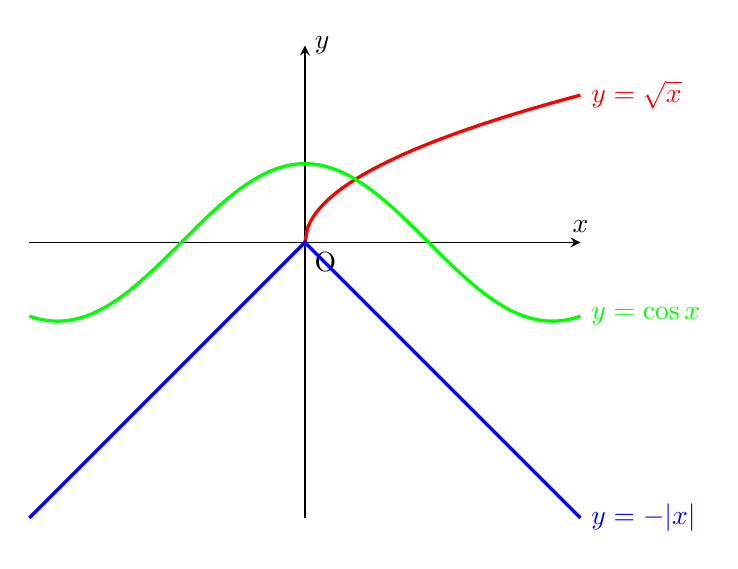
\begin{tikzpicture}
 \draw[->,>=stealth,semithick] (-3.5,0)--(3.5,0)node[above]{$x$}; %x軸
 \draw[->,>=stealth,semithick] (0,-3.5)--(0,2.5)node[right]{$y$}; %y軸
 \draw (0,0)node[below right]{O}; %原点
 \draw[red,very thick,samples=100,domain=0:3.5] plot(\x,{sqrt(\x)})node[right]{$y=\sqrt{x}$};
 \draw[blue,very thick,domain=-3.5:3.5] plot(\x,{-abs(\x)})node[right]{$y=-|x|$};
 \draw[green,very thick,samples=100,domain=-3.5:3.5] plot(\x,{cos(\x r)})node[right]{$y=\cos{x}$};
\end{tikzpicture}
